 \documentclass[book.tex]{subfiles}
\begin{document}

\section{Smooth scrolling}
\label{section:adaptive_tile_refresh}
Performing a full-screen redraw per frame would kill the CPU, as it would need to update all pixels of all four EGA planes. There is no way to maintain a 60Hz framerate while refreshing the whole screen. If we were to run the following code, which simply fills all memory banks, it would run at 5 frames per seconds.\\

\par
\begin{minipage}{\textwidth}
  \lstinputlisting[language=C]{code/write_ega.c}
  \end{minipage}
  \label{ega_write}

\par
So how did they create a smooth scrolling game with these limitations? By using some EGA hardware tricks and by changing only that part of the screen that has changed.
\pagebreak



\subsection{EGA Virtual Screen and Pel Panning}
\label{section:EGA_virtual_screen}

The EGA adds a powerful twist to linear addressing: the logical width of the virtual screen in VRAM memory need not to be the same as the physical width of the screen display. The programmer is free to define a virtual screen width of up to 4096 pixels and then use the physical screen as a window onto any part of the virtual screen. What's more, a virtual screen can have any logical height up to the capacity of the VRAM memory. The code below illustrates how to change the logical width.\\

\begin{minipage}{\textwidth}
  \lstinputlisting[language=C]{code/SCREEN_WIDTH.ASM}
  \end{minipage}
  \label{ega_pel_pan}
  \par

The area of the virtual screen displayed at any given time is selected by setting the display memory address at which to begin fetching video data. This is set by way of the CRTC Start Address register. The default address is \cw{A000:0000h}, but the offset can be changed to any other number. \\

\begin{minipage}{\textwidth}
  \lstinputlisting[language=C]{code/EGA_SET_ADDRESS.ASM}
  \end{minipage}
  \label{ega_set_address}
  \par


\par
Panning down a scan line requires only that the CRTC start address is increased by the logical width. Horizontal panning is possible by increasing the start address by one byte. In EGA's planar graphics modes, the eight bits in each byte of video RAM correspond to eight consecutive pixels on-screen. That means the screen moves horizontally in steps of 8 pixels, which is coarse, not smooth scrolling. Luckily there is another register we can use to resolve this.\\

\begin{figure}[H]
\centering
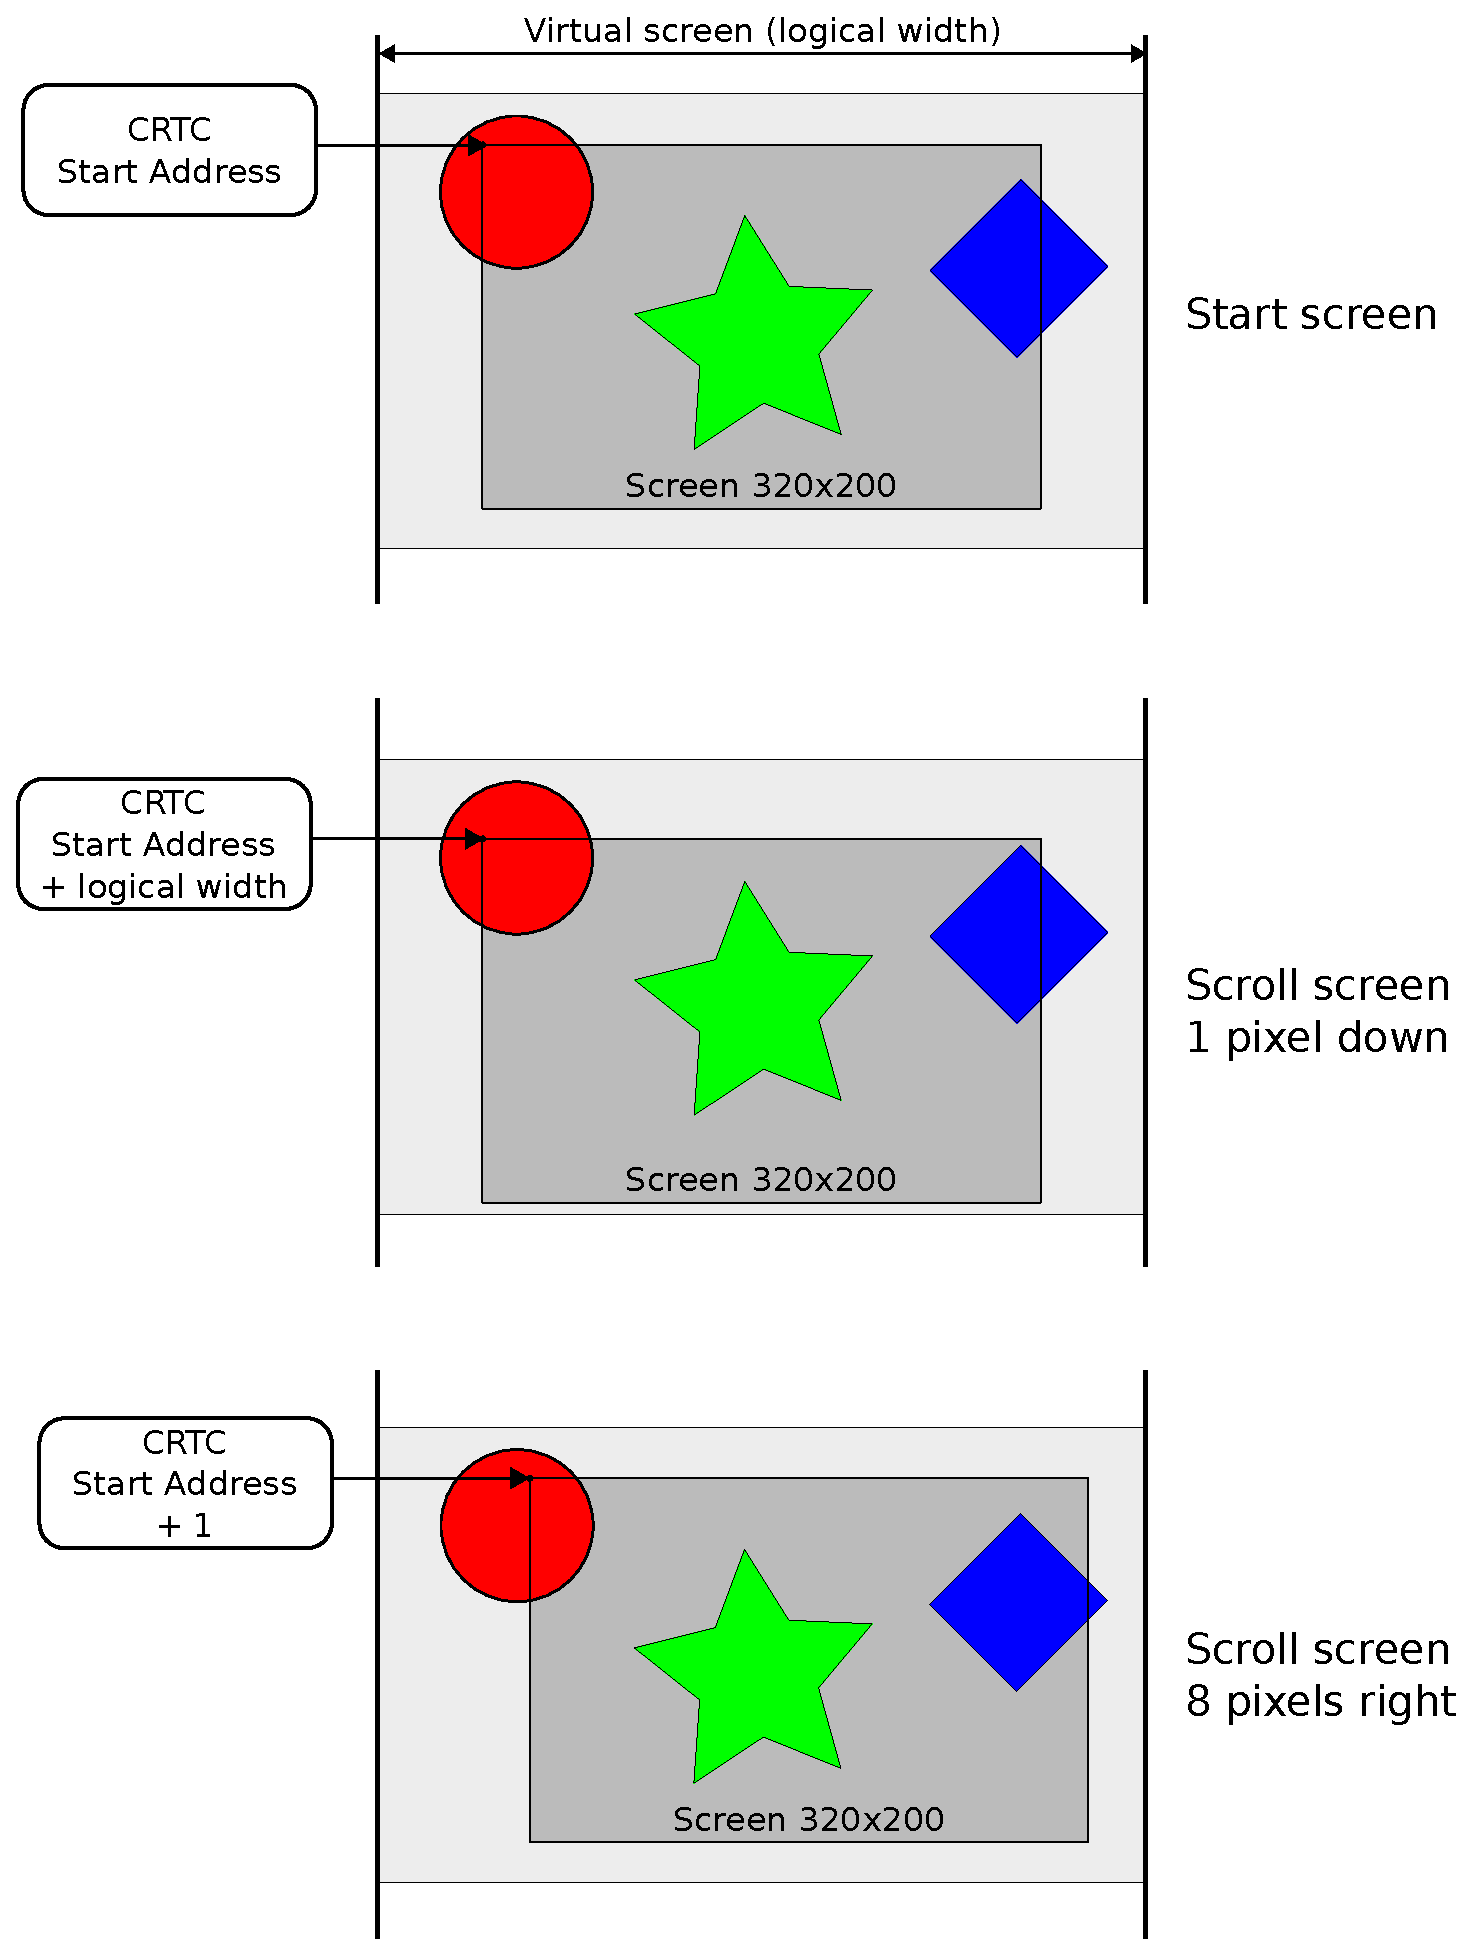
\includegraphics[width=0.9\textwidth]{imgs/drawings/virtual_screen.eps}
\caption{EGA screen scrolling by updating the CRTC Start Address.}
\label{fig:tile_refresh}
\end{figure}



\subsection{Horizontal Pel Panning}
Smooth horizontal pixel scrolling of the screen is provided by the "Horizontal Pel Panning" register in the Attribute Controller (ATC). Up to 7 pixels' worth of single pixel panning of the displayed image to the left is performed by increasing the register from 0 to 7. \\
\par

There is one annoying quirk about programming the Attribute Controller: when the ATC Index register is set, only the lower five bits (bits 0-4) are used as the internal index. The next most significant bit, bit 5, controls the source of the video data send to the monitor by the EGA card. When bit 5 is set to 1, the output of the color palette controls the displayed pixels; this is normal operation. When bit 5 is 0, video data doesn't come from the color palette, and the screen becomes a solid color. To ensure the ATC index register is restored to normal video, we must set bit 5 to 1 by writing \cw{20h} to the register.\\ 

\begin{minipage}{\textwidth}
  \lstinputlisting[language=C]{code/EGA_PELPAN.ASM}
  \end{minipage}
  \label{ega_pel_pan}
  \par

\subsection{Bring it all together}


\par
Smooth horizontal on EGA should be viewed as adjusting the CRTC Start Address and fine horizontal adjustments in the 8-pixel range. The scrolling is achieved by the following steps:
\begin{itemize}
  \item calculate the panning in pixels for both x- and y-direction
  \item the smooth y-panning is defined by adding \cw{logical width * y} to the CRTC start address
  \item increase the CRTC start address width \cw{x/8} bytes for coarse horizontal scrolling.
  \item the horizontal fine tuning is then adjusted by \cw{x mod 8} using horizontal pel panning
\end{itemize}




\begin{figure}[H]
\centering
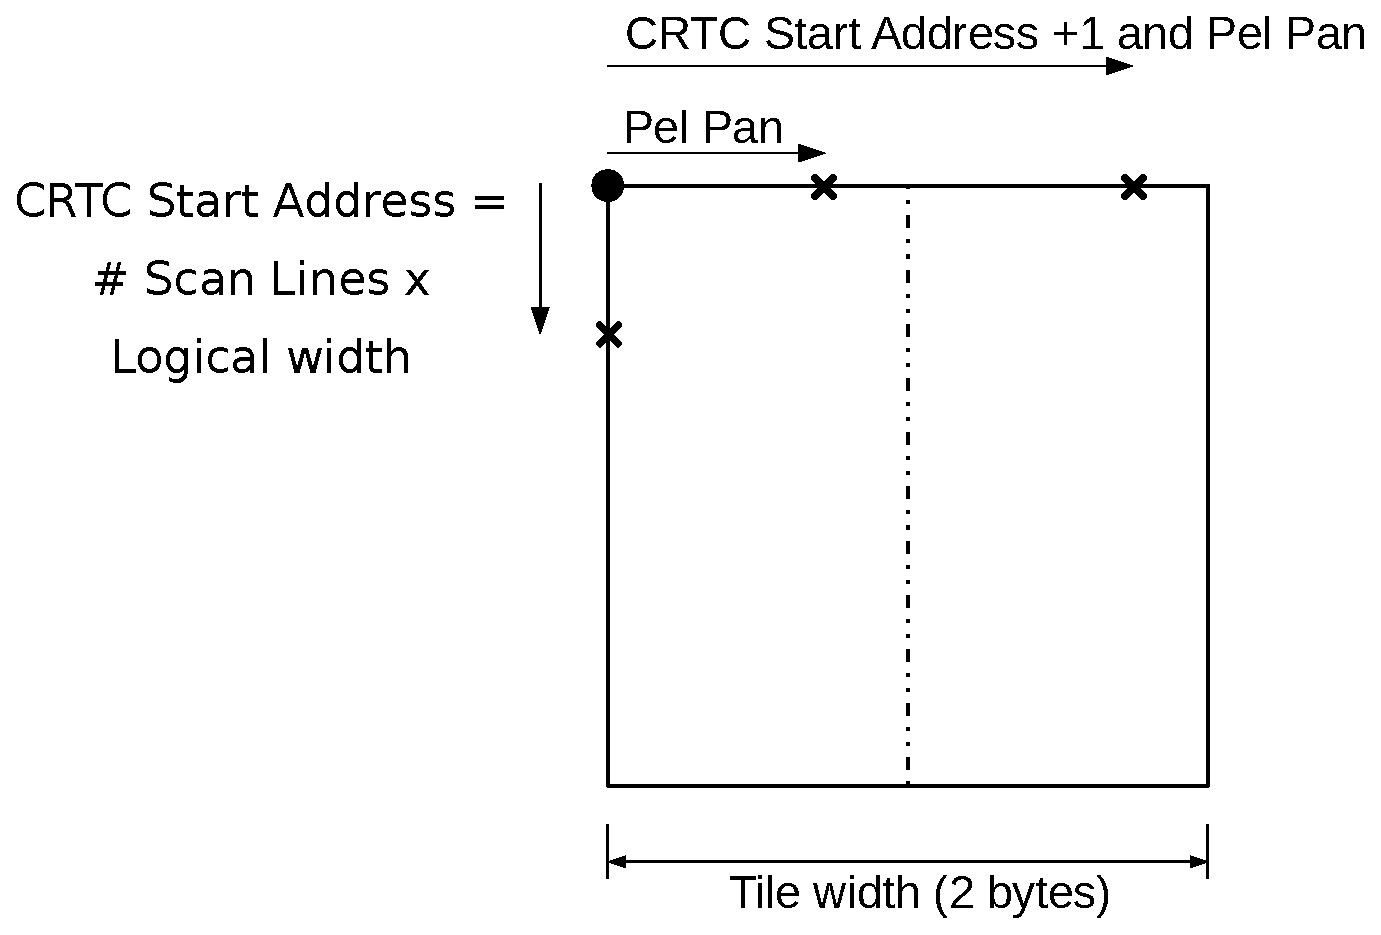
\includegraphics[width=0.6\textwidth]{imgs/drawings/Tile_Refresh.eps}
\caption{Smooth scrolling in EGA.}
\label{fig:tile_refresh}
\end{figure}

\section{Adaptive Tile Refreshment}
So far, we have built a virtual screen in VRAM allowing smooth one pixel moves in both axes using only EGA registers. But once it reaches an edge, the virtual screen must be reset. And it cannot be a full screen redraw because it would drop the framerate to 5fps.\\


\begin{figure}[H]
\centering
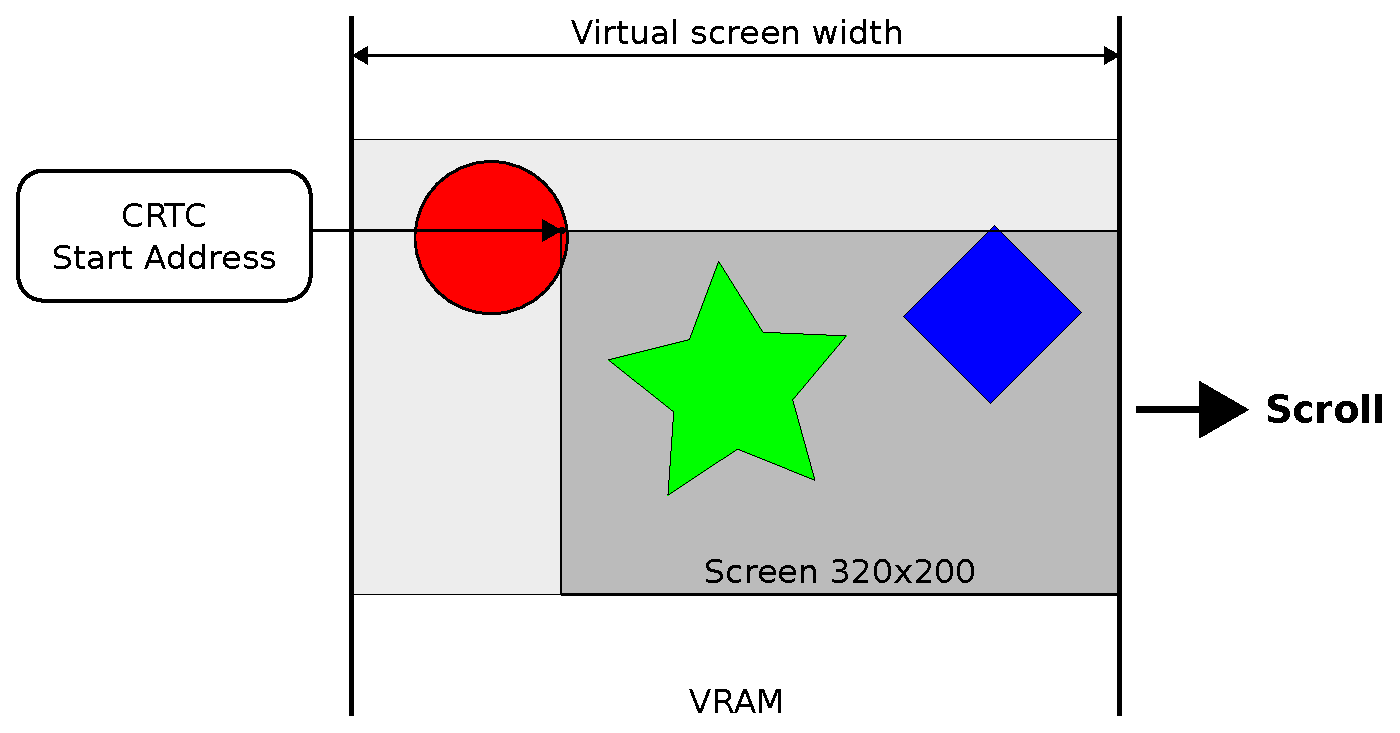
\includegraphics[width=0.7\textwidth]{imgs/drawings/screen_edge.eps}
\caption{Screen reaching the edge of virtual screen.}
\label{fig:screen_edge}
\end{figure}

\par
An option to resolve screen refresh is loading the entire level into VRAM memory and setting the logical width to the level width. By simply updating the CRTC Start Address and Horizontal Pel Panning registers, the game scrolls smoothly through the virtual screen. Unfortunately, a level won't fit into the VRAM. The first level, \textit{Horsh Radish Hill}, is 2176 pixels wide and 592 pixels high, which means a total of 2176*592/2 = 644KB is required to store the entire level in VRAM. Since we only have 256KB available, this is not a feasible option. \\


\textbf{\underline{Trivia :}} At the time of writing this book, most video cards contain more tha 1GB VRAM, sufficient to store all Commander Keen levels at once in VRAM. \\

\par
This is where John Carmack's invention starts. The scrolling engine is based on a simple yet powerful technology called \textit{Adaptive Tile Refreshment (ATR)}. The core idea is to refresh only those areas of the screen that need to change. The screen is divided into tiles of 16x16 pixels. On a screen with 320x200 pixels, it means a grid of 20x13 tiles (actually it is 12.5 tiles high, but we round to full tiles). \\

\par
Let's look at \textit{Commander Keen 1: Marooned on Mars} in Figure \ref{fig:keen_difference}. This is the first level of Marooned, immediately to the right of the crashed Bean-with-Bacon Megarocket. The first figure is the start of the level, the second figure is after Keen has scrolled one tile (16 pixels) to the right through the world. They look almost identical to the naked eye, don't they? \\

\par
Now, if we perform a difference on both images, you can see which tiles need to be changed upon screen refresh. The trick behind the scrolling is to only redraw tiles that actually changed after panning 16 pixels (one tile). For matching tiles there is nothing to do and they are skipped entirely. In Figure 4.21, there are large swathes of constant background tiles. In total, only 69 tiles out of the 260 tiles need to be refreshed, which is 27\% of the screen!





\pagebreak
\begin{figure}[H] 
  \centering 
  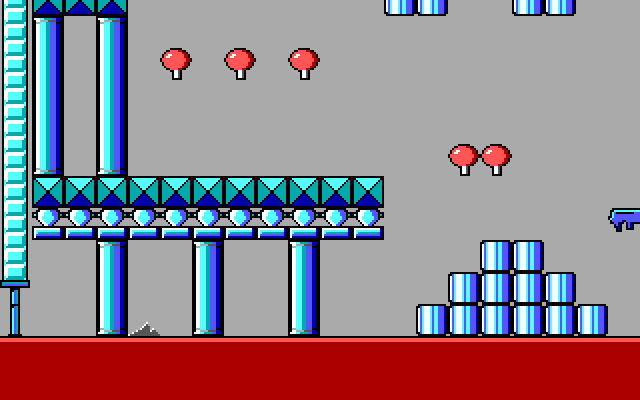
\includegraphics[width=.6\textwidth, frame]{screenshots_300dpi/game/keen-screen1.png}
\end{figure}
\begin{figure}[H] 
  \centering 
  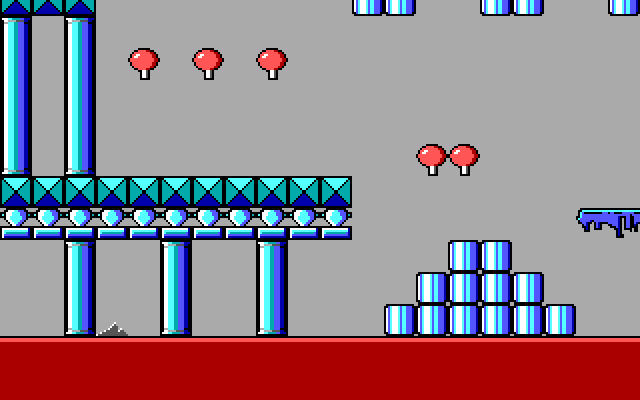
\includegraphics[width=.6\textwidth, frame]{screenshots_300dpi/game/keen-screen2.png}
\end{figure}
\begin{figure}[H] 
  \centering 
  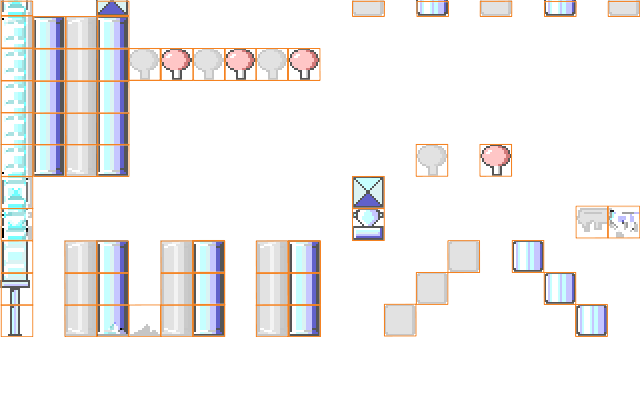
\includegraphics[width=.6\textwidth, frame]{screenshots_300dpi/game/keen-difference.png}
  \caption{Start of the world, moved one tile to the right and difference.}
  \label{fig:keen_difference}
\end{figure}
\pagebreak

\section{ATR in action: Commander Keen 1-3}
This section explains how ATR is working for the first three episodes of Commander Keen. We can only explain how the algorithm is working without code examples, since the only released code is Keen Dreams which is using a different, improved algorithm which will be explained later\footnote{https://retrocomputing.stackexchange.com/questions/22175/what-is-adaptive-tile-refresh-in-the-context-of-commander-keen}.\\

\par
Even if the screen is not scrolling, tile refreshes are required to support sprite and tile animations. Since moving a sprite in this way involves first erasing it and then redrawing it, the image of the erased sprite may be visible briefly, causing flicker. This is where double buffering comes in: setting up a second buffer into which the code can draw while the first buffer is being shown on screen, which is then switched out during screen refresh. This ensures that no frame is ever displayed mid-drawing, which yields smooth, flicker-free animation.\\

Now, let's have a closer look at the EGA VRAM setup. The video memory is organized into three virtual screens:
\begin{itemize}
\item Page 0 and 1, which are used to switch between buffer and visible screen
\item A master page containing a static page, which is copied to the buffer memory when performing the screen refresh.
\end{itemize}



\begin{figure}[H]
\centering
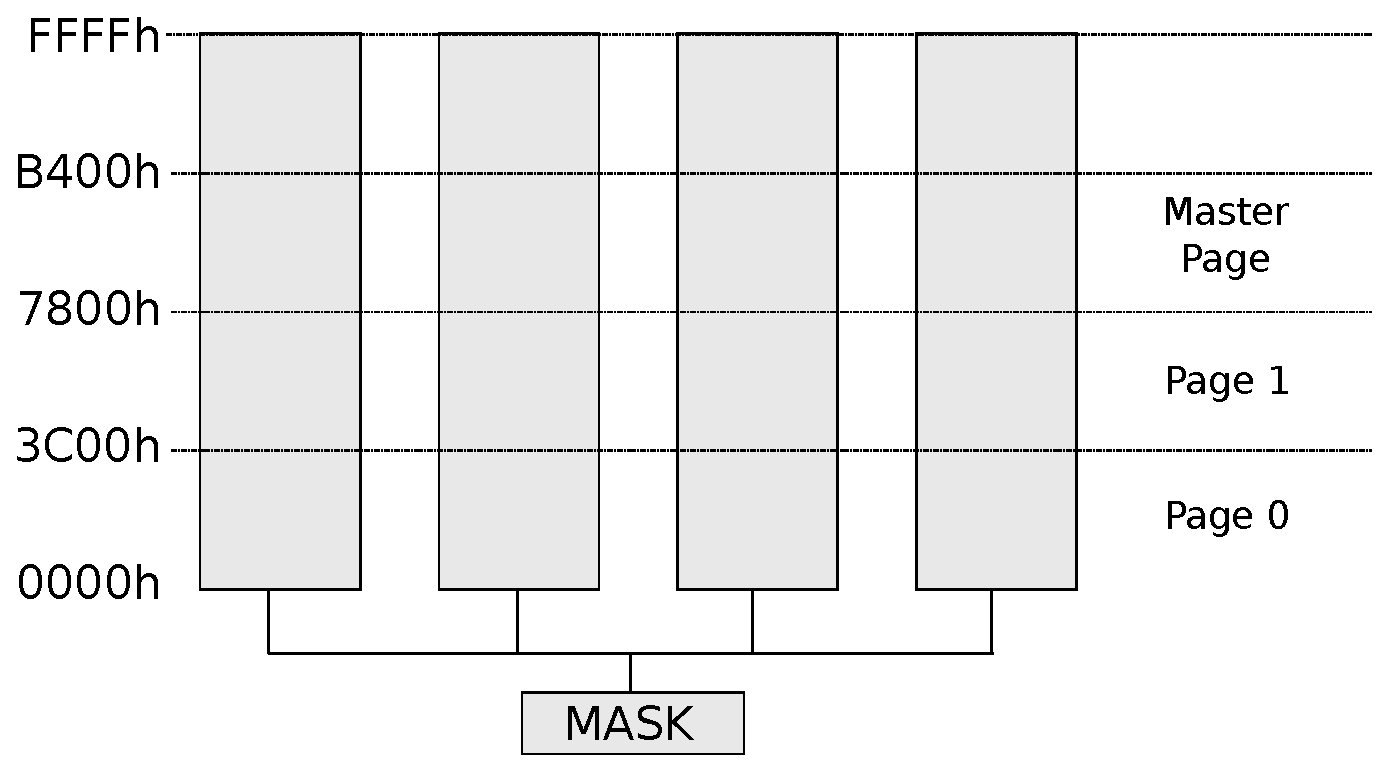
\includegraphics[width=\textwidth]{imgs/drawings/ega_ram_architecture.eps}
\caption{Virtual screen layout on EGA card.}
\label{fig:ega_ram_arch}
\end{figure}

\par
The EGA screen in mode \cw{0xD} has a resolution of 320x200 pixels, which is 40x200 bytes. Let's extend the height by 8 bytes to have a height of 208 pixels, so the screen fits nicely in 20x13 tiles of 16x16 pixels. By making the virtual screen one tile higher (16 bytes) and one wider (2 bytes) on each side of the screen, the engine can scroll up to 16 pixels to any direction of the screen without any tile refresh, by simply adjusting the CRTC Start Address and Pel Pan registers.\\

\begin{figure}[H]
\centering
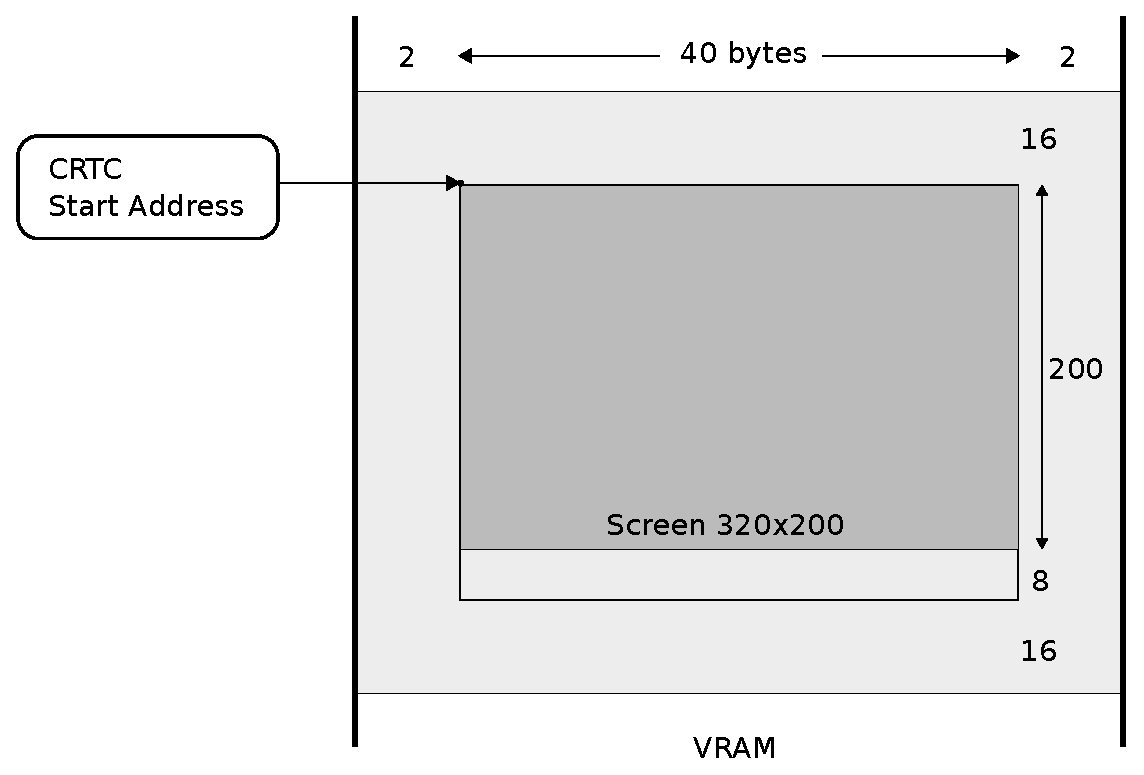
\includegraphics[width=0.9\textwidth]{imgs/drawings/ATR_virtual_screen.eps}
\label{fig:atr_virtual screen}
\end{figure}




\par
Each virtual screen has a size of 44*240=10,560 bytes per memory bank, in total 42KB. So within a 256KB EGA card there is enough VRAM available to keep all three virtual screens in memory. The page that is actually displayed at any given time is selected by setting the CRTC Start Address register at which to begin fetching video data.\\

\par
For both the buffer and visible screen a tile index array is created to maintain which tiles are changed since last refresh. Now six stages are involved in refreshing the screen:
\begin{enumerate}
\item Check if the player has moved one tile in any direction and mark all sprites that have moved or need to be removed.
\item Validate which tiles have changed and copy these respective tiles to the master page and mark the tiles in both tile index arrays. Then also copy and mark any animated tiles.
\item Refresh the buffer page by scanning the tile index array. If a tile is marked, copy the tile from the master page to the buffer page.
\item Iterate through the sprite removal list and copy corresponding image block from the master page to buffer page. 
\item Iterate through the sprite list and copy corresponding sprite from memory to the buffer page.
\item Switch the view and buffer page by adjusting the CRTC Start Address and Pel Panning registers.
\end{enumerate}



In the next six screenshots, we take you step-by-step through each of the stages. The player has reached the edge of the virtual screen and moves further to the right. \\





\begin{figure}[H]
\centering
 \fullimage{/game/Keen_ATR_1-3_a.png}
 \caption{Step 1: Scroll screen to the right}
 \label{fig:kc1_3_start}
\end{figure}

\begin{figure}[H]
\centering
 \fullimage{/game/Keen_ATR_1-3_step1.png}
 \caption{Step 2: Update changed tiles in master page, marked in dark grey}
 \label{fig:kc1_3_update_masterscreen}
\end{figure}

The engine keeps track of which tile IDs are in the virtual screen. Since the engine only refresh at tiles size granularity, it can determine extremely fast what has changed on the screen by comparing tile IDs. If the tile number has changed, the tile is updated by copying tile data from RAM into the corresponding location of the VRAM master page. The changed tiles are marked with a '1' in both tile arrays, which means it needs to be updated upon next refresh.

\begin{figure}[H]
\centering
 \fullimage{/game/Scroll_KC1-3_1-tile_mem2master.png}
 \caption{Mark all changed tiles with '1' in both tile buffer and tile view array.}
 \label{fig:kc1_3_update_refresh_img_1}
\end{figure}


\pagebreak

\begin{figure}[H]
\centering
 \fullimage{/game/Scroll_KC1-3_1-master2buffer.png}
 \caption{Step 3 and 4: Copy tiles from master to buffer page and remove sprites}
 \label{fig:kc1_3_update_remove}
\end{figure}

The next step is to scan all tiles in the tile buffer array and for each tile marked as '1', copy the tile from master to buffer page.\\
\par
If a sprite has moved or disappeared, the latest sprite location is added to the block erase list. For each block in this erase list, erase the sprite by copying the width and height of the sprite block (marked in green in Figure \ref{fig:kc1_3_update_remove}) from the master to the buffer page, and mark the corresponding tiles only in the tile buffer array with a '2'.

\begin{figure}[H]
\centering
 \fullimage{/game/Scroll_KC1-3_1-tile_master2buffer.png}
 \caption{Mark removed sprites with '2' in tile buffer array only.}
 \label{fig:kc1_3_tile_update_remove}
\end{figure}


\pagebreak

\begin{figure}[H]
\centering
 \fullimage{/game/Scroll_KC1-3_1-sprite2buffer.png}
 \caption{Step 5: Scan sprite list and copy sprite onto buffer page}
 \label{fig:kc1_3_update_sprite}
\end{figure}

Next, the engine scans the sprite list. Validate if the sprite is in the visible part of the view port and copy the sprite image to the buffer page. Mark the corresponding tiles in the tile buffer array with a '3'.

\begin{figure}[H]
\centering
 \fullimage{/game/Scroll_KC1-3_1-tile_sprite2buffer.png}
 \caption{Mark new sprites locations with '3' in tile buffer array only.}
 \label{fig:kc1_3_tile_update_sprite}
\end{figure}


\pagebreak


\begin{figure}[H]
\centering
 \fullimage{/game/Scroll_KC1-3_1-final.png}
 \caption{Step 6: Swap buffer and view page}
 \label{fig:kc1_3_update_final}
\end{figure}


In the last step, point the visible screen to the buffer page by updating the CRTC start address and horizontal Pel Panning register. Finally, the tile buffer array is cleared to '0' and both arrays are swapped (so tile buffer becomes the tile view). Then step 1 is repeated. \\
\par
Note that after swapping, the tile buffer array has marked all tiles that have changed from scrolling the screen. This makes sense, as the current buffer page is not yet refreshed (it was displayed in the previous refresh cycle, and we never update the view page). 

\begin{figure}[H]
\centering
 \fullimage{/game/Scroll_KC1-3_1-tile_final.png}
 \caption{Clear tile buffer array and swap tile arrays.}
 \label{fig:kc1_3_tile_final}
\end{figure}


\pagebreak

\begin{figure}[H]
\centering
 \fullimage{/game/Scroll_KC1-3_1_final.png}
 \caption{Step 6: Swap buffer and screen page}
 \label{fig:kc1_3_update_final}
\end{figure}

Step 2 and 3 (except for the animated tiles) only needs to happen if Commander Keen is moving more than 16 pixels, where step 4 and 5 normally needs to happen for each refresh.
So the number of drawing operations required during each refresh is controllable by the level designer. If they choose to place large regions of identical tiles (the large swathes of constant background), less redrawing (meaning: less redrawing in step 2 and 3) is required.

\pagebreak




\subsection{Wrap around the EGA Memory}
\label{section:wrap_ega_memory}
\label{section:optimize_tile}
John Carmack explored what would happen if you push the virtual screen over the 64kB border (address \cw{0xFFFF}) in video memory. It turned out that the EGA continues the virtual screen at \cw{0x0000}. This means you could wrap the virtual screen around  the EGA memory and only need to add a stroke of tiles on one of the edges when Commander Keen moves more than 16 pixels.\\
\par
\begin{figure}[H]
  \centering
  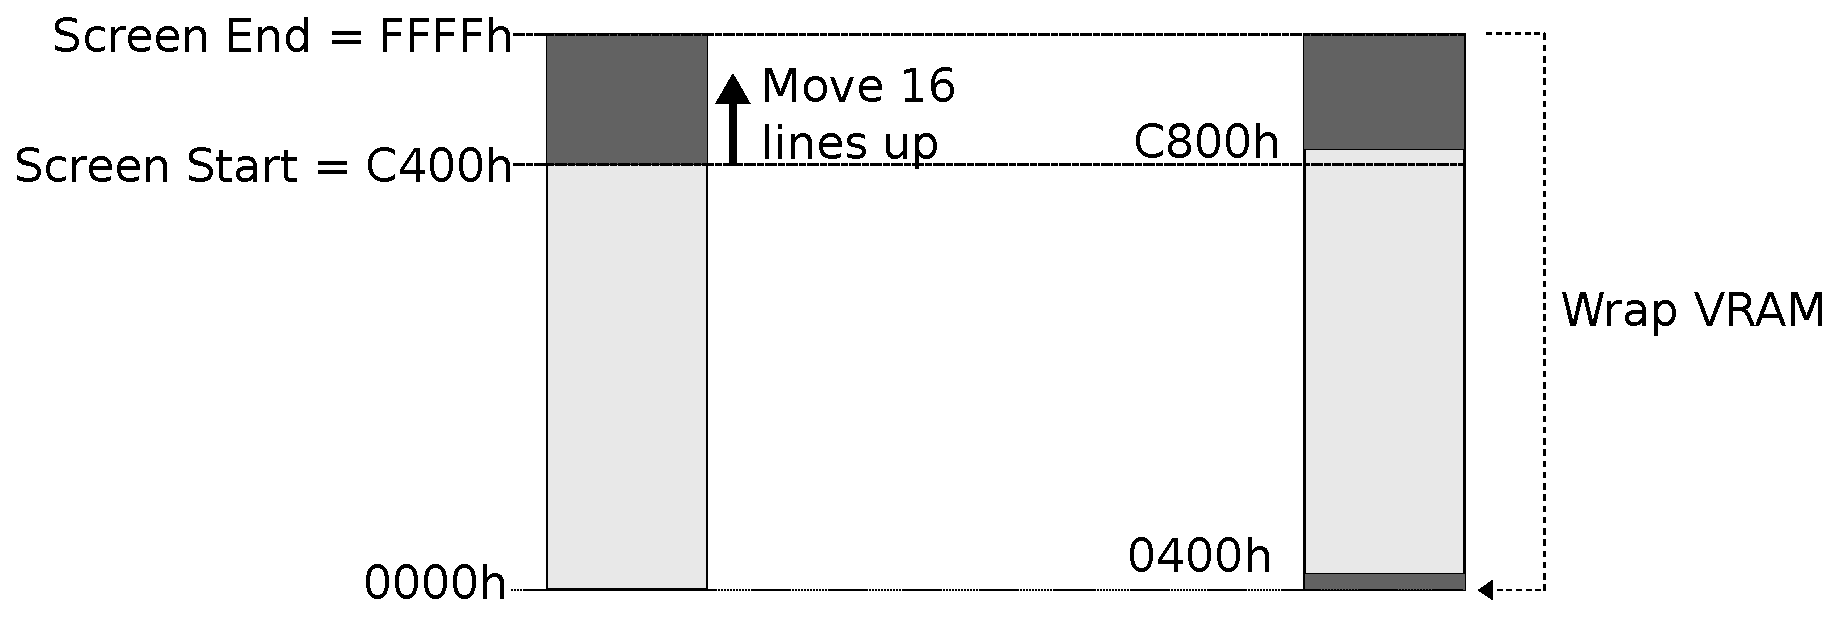
\includegraphics[width=\textwidth]{imgs/drawings/ega_wrapping.eps}
  \label{fig:ega_wrapping}
  \caption{Wrap virtual screen around the EGA memory}
\end{figure}

\par
\begin{fancyquotes}
I finally asked what actually happens if you just go off the edge [OF THE VRAM]?\\

If you take your [CRTC] start and you say OK, I can move over and I get to what should be the bottom of the memory window. [...] What happens if I start at 0xFFFE at the very end of the 64k block? It turns out it just wraps back around to the top of the block.\\

I'm like oh well this makes everything easy. You can just scroll the screen everywhere and all you have to draw is just one new line of tiles.\\

It just works. We no longer had the problem of having fields of similar colors. It doesn't matter what you're doing, you could be having a completely unique world and you're just drawing the new strip.\\
\par
\textbf{John Carmack\protect\footnotemark}
\end{fancyquotes}\\
\addtocounter{footnote}{-1}
\stepcounter{footnote}
\footnotetext{An explanation further elaborated during an interview with Lex Fridman in 2022.}
\par

There was however an issue with the introduction of Super VGA cards, which had typically more than 256kB RAM\footnote{In 1989 the VESA consortium standardized an API to use Super VGA modes in a generic way. One of the first modes was 640x480 at 256 colors requiring at least 256kB RAM, which from a hardware constraint resulted in 512kB.}. This resulted in crippled backwards compatibility and the wrapping around \cw{0xFFFF} did not work anymore on these cards. \\
\par
There is a simple way to resolve this issue. As you can see in Figure \ref{fig:ega_ram_arch} on page \pageref{fig:ega_ram_arch}, the space between \cw{0xB400} and \cw{0xFFFF} is not used and contains enough space for another virtual screen. Each screen buffer has a size of \cw{0x3C00} in each memory bank. In case the start address is between \cw{0xC400} and \cw{0xFFFF} the corresponding screen is copied to the opposite end of the buffer, as illustrated in Figure \ref{fig:page_wrapping}.\\

\par

\begin{fancyquotes}
I was in a tough position. Do I have to track every single one of these [SUPER VGA CARDS] and it was a madhouse back then with 20 different video card vendors with all slightly different implementations of their non-standard functionality. Either I needed to natively program all of the cards or I kind of punt. I took the easy solution of when you finally did run to the edge of the screen I accepted a hitch and just copied the whole screen up.\\
\par
\textbf{John Carmack}
\end{fancyquotes}\\

\par
\begin{figure}[H]
\centering
\begin{subfigure}{.5\textwidth}
  \centering
  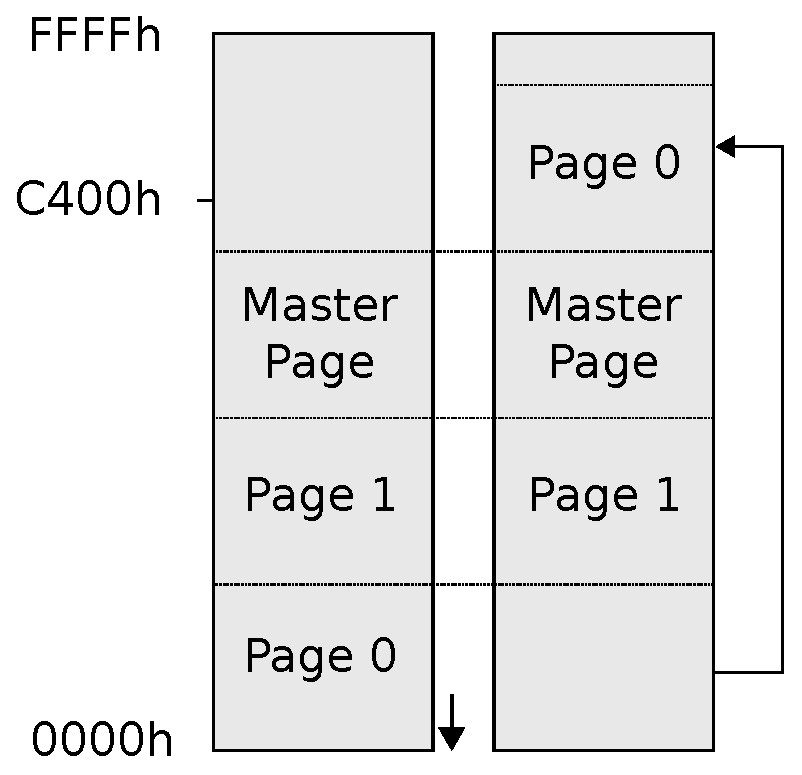
\includegraphics[width=.9\textwidth]{imgs/drawings/Page_down_switch.eps}
  \caption*{Virtual pages moved down}
  \label{fig:page0_down}
\end{subfigure}%
\begin{subfigure}{.5\textwidth}
  \centering
  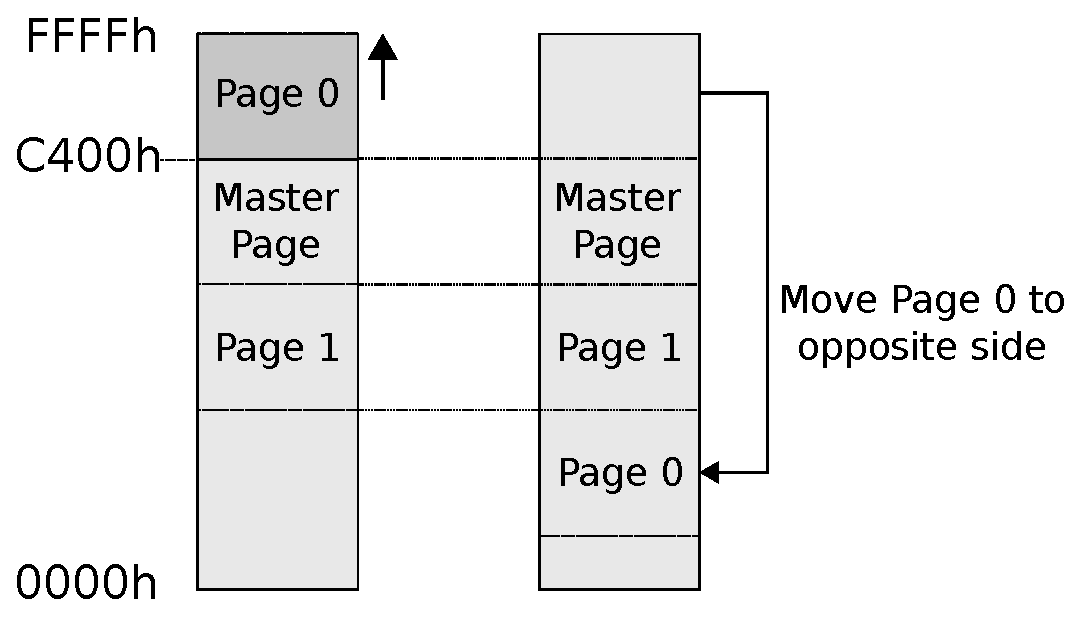
\includegraphics[width=.9\textwidth]{imgs/drawings/Page_up_switch.eps}
    \caption*{Virtual pages moved up}
  \label{fig:page0_up}
\end{subfigure}
\caption{Move screen to opposite end of VRAM buffer}
\label{fig:page_wrapping}
\end{figure}



\par
\begin{minipage}{\textwidth}
  \lstinputlisting[language=C]{code/wrap_page_buffer.c}
  \end{minipage}
  \label{ega_refresh}
  \par
But how can we copy four VRAM planes fast enough, without noticing any performance hit? As explained in Section \ref{section:ega_memmap} each pixel is encoded by four bits, which are spread across the four EGA banks. Since all write operations are one byte wide, it is not hard to imagine the difficulty in plotting a single pixel without changing the others stored in the same byte. One would have to do four read, four xor, and four writes.\\
\par
 Since the designers of the EGA were not complete sadists, they added some circuitry to simplify this operation. For each bank, they created a latch placed in front of a configurable ALU.\\
\par
 \begin{figure}[H]
\centering
 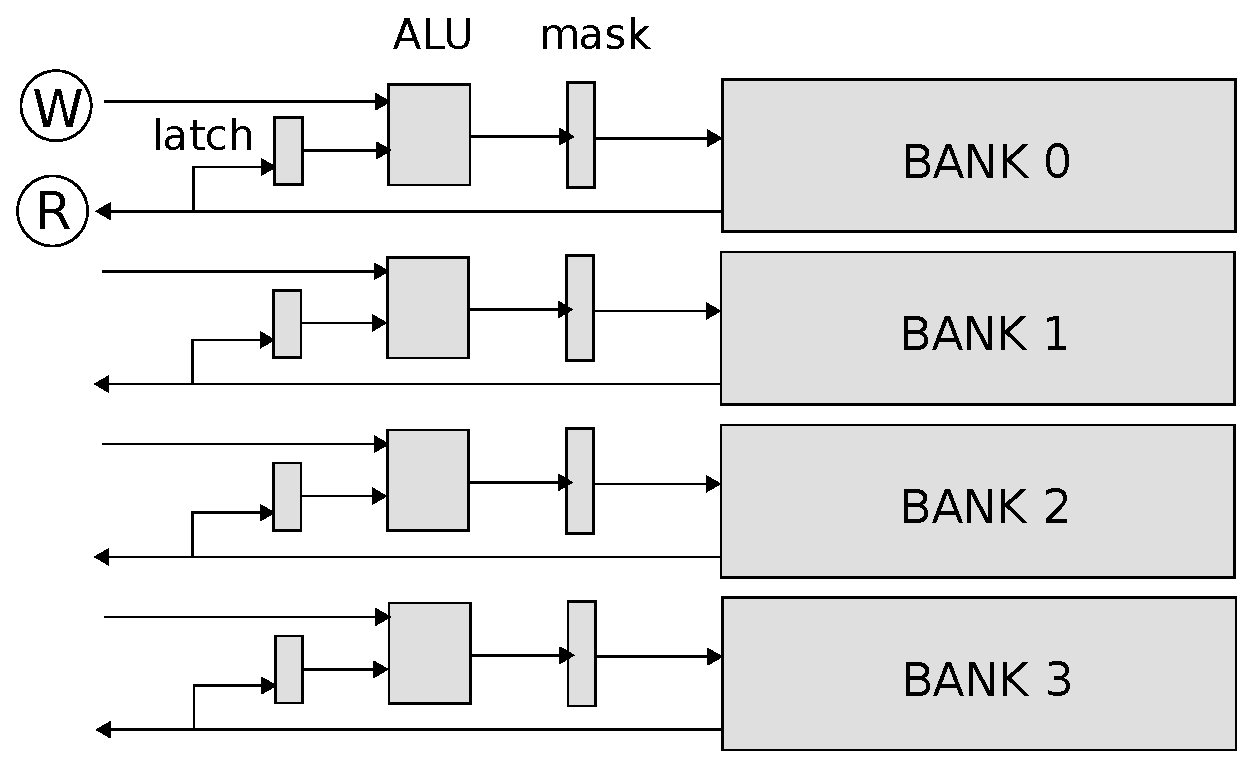
\includegraphics[width=\textwidth]{imgs/drawings/latches.eps}
 \caption{Latches memorize read operations from each bank. The memorized value can be used for later writes.}
 \end{figure}
With this architecture, each time the VRAM is read \circled{R}, the latch from the corresponding bank is loaded with the read value. Each time a value is written to the VRAM \circled{W}, it can be composited by the ALU using the latched value and the written value. This design allowed mode \cw{0Dh} programmers to plot a pixel easily with one read, one ALU setup, and one write instead of four reads, 4 xors, and 4 writes.\\
\par
By getting a little creative, the circuitry can be re-purposed. The ALU in front of each bank can be setup to use only the latch for writing. With such a setup, upon doing one read, four latches are populated at once and four bytes in the bank are written with only one write to the RAM. This system allows transfer from VRAM to VRAM 4 bytes at a time. Now it is possible to copy the entire buffer fast enough, without notifying any performance impact.\\
\par
\begin{minipage}{\textwidth}
  \lstinputlisting[language=C]{code/EGA_LATCH_COPY.ASM}
  \end{minipage}
  \label{ega_latch_copy}
  \par

To take full advantage of this optimization, the refresh algorithm maintains a list of tiles that are already copied on the master page via \cw{tilecache} variable. If a tile is already on the master page the algorithm copies the tile from that location to its destination instead of the RAM location in memory, saving the four separated writes to each memory plane.\\



\pagebreak

\subsection{Adaptive tile refreshment in Commander Keen in Keen Dreams} \label{section:scroll_refresh_dreams}

The EGA memory wrapping results in an improved, more simplified Adaptive Tile Refreshment algorithm. The following six steps take place, where \cw{*screenstart[]} are pointers to the starting address (upper-left pixel) of the viewports in VRAM and \cw{*updatestart[]} are pointers to the tile view and buffer arrays.
\begin{enumerate}
\item Check if the player has moved one tile in any direction.
\item In case the player moved one tile, move the \cw{*screenstart[]} and \cw{*update[]} pointers accordingly and copy the new column or row of tiles to the master page and flag this new column/row of tiles to be updated in the next refresh for both pages. 
\item Refresh the buffer page by scanning all tiles in the tile buffer array. If a tile is flagged for update, copy the tile from the master page to the buffer page.
\item Iterate through the sprite removal list and copy corresponding image block from master page to buffer page. 
\item Iterate through the sprite list and copy corresponding sprite image block from RAM to buffer page.
\item Switch the view and buffer page by adjusting the CRTC Start Address and Pel Panning register.
\end{enumerate}

As you can see, only step 2 is different from Commander Keen 1-3, the rest of the steps are the same. In the example below the screen is forced to scroll to the left.


\begin{figure}[H]
\centering
 \scaledimage{0.85}{/game/Scroll_KC4_6_1.png}
 \caption{Step 1: Scroll screen to the left}
 \label{fig:kc4_6_start}
\end{figure}

\pagebreak

\begin{figure}[H]
\centering
 \fullimage{/game/Scroll_KC4-6_1-mem2master.png}
 \caption{Step 2 and 3: Shift screen pointer and add column to VRAM}
 \label{fig:kc4_6_add_column}
\end{figure}


First decrease the \cw{*screenstart[]} pointers by 2 bytes (1 tile). Then copy a left-column of new tiles from RAM to the master page.\\
\par
In parallel both tile array pointers are decreased by one byte and each tile on the left border in both buffer arrays is marked with '1', so it is updated upon the next refresh.
Finally, the most right column (which is now outside the view port) is marked with a '0'.

\begin{figure}[H]
\centering
 \fullimage{/game/Scroll_KC4-6_1-tile_master2buffer.png}
 \caption{Mark new column in both tile buffer and display array.}
 \label{fig:kc4_6_tile_final}
\end{figure}


\begin{figure}[H]
\centering
 \fullimage{/game/Scroll_KC4-6_1-view_buffer.png}
 \caption{Step 3 to 6: Update buffer page with tile animations and sprites}
 \label{fig:kc4_6_update_buffer}
\end{figure}


Just like before, we copy the animated tiles from RAM to master page and mark them as '1' in both tile arrays. Then we scan all '1' and copy those tiles from master to buffer page. The remaining steps are the same as before, meaning erasing and copying sprites to the buffer page and finally swap the buffer and view pages.

\begin{figure}[H]
\centering
 \fullimage{/game/Scroll_KC4-6_1-tile_view_buffer.png}
 \caption{Final tile arrays layout after buffer page is updated.}
 \label{fig:kc4_6_update_array}
\end{figure}

\par
\textbf{\underline{Trivia :}} The removal blocks which are marked '2' in the tile buffer array are nowhere used in the engine.\\
  \par
\pagebreak

\begin{figure}[H]
\centering
 \scaledimage{0.85}{/game/Scroll_KC1-4-6_final.png}
 \caption{Step 7: Updated screen after swapping buffer and screen page}
 \label{fig:k4_6_update_final}
\end{figure}


Since we only need to update one border, the engine needed to update only 6\% of the screen!\\


\par
\begin{minipage}{\textwidth}
  \lstinputlisting[language=C]{code/refresh.c}
\end{minipage}
\label{state_type}
\par

Now we can also explain why the tile buffer and view arrays are 2 tiles wider on all sides than the view port as illustrated in Figure \ref{fig:screen_setup}. Let's take the situation where the screen scrolls to the top-left, meaning 1 tile left and 1 tile up as illustrated in Figure \ref{fig:buffer_tile_move_1}. Both \cw{*updatestart} pointers are updated and tiles are marked as '1'. After completing all tile refresh steps, the buffer page is updated on places where the tile buffer array is marked '1'. \\
\par
After the view page is swapped with the buffer page, the \cw{*updatestart[otherpage]} pointer is cleared and the array is reset to '0'. However, the \cw{*updatestart[screenpage]} is not cleared nor reset since we did not update the view page (we only updated the buffer page).\\
\begin{figure}[H]
  \centering
  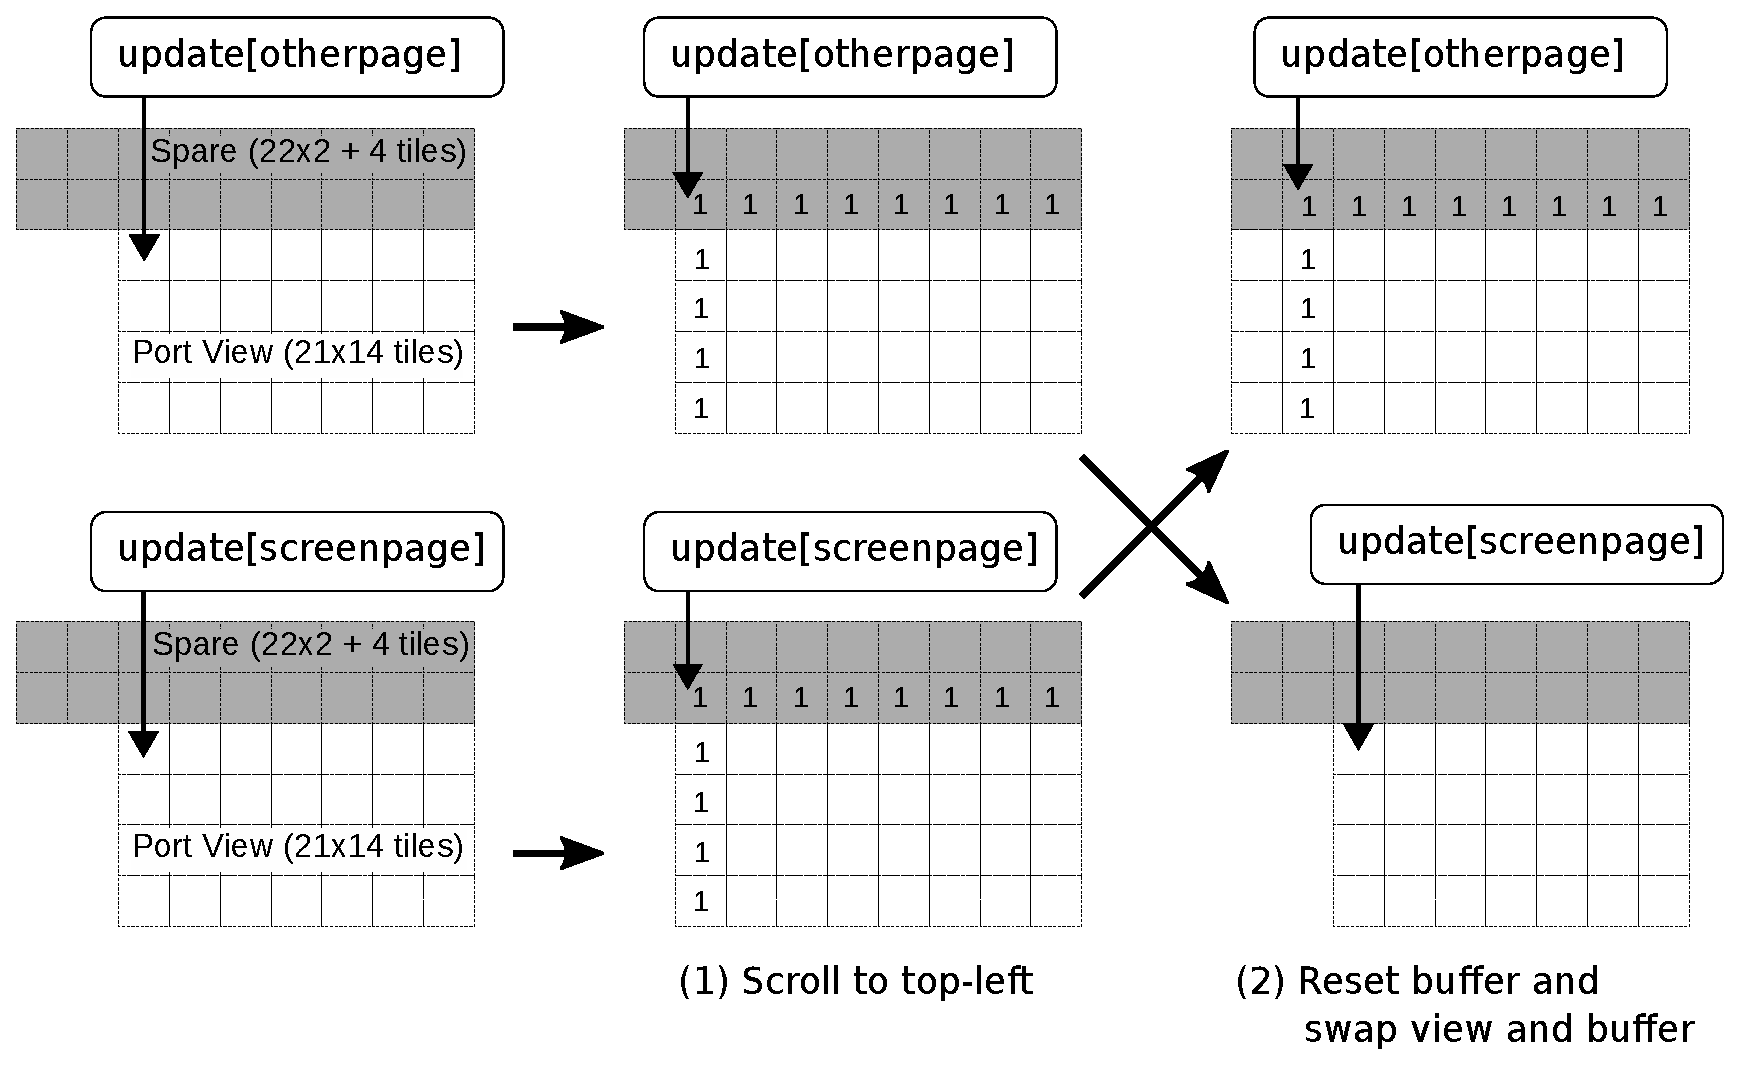
\includegraphics[width=0.85\textwidth]{imgs/drawings/buffer_tile_move_1.eps}
  \caption{scroll to top-left tile.}
  \label{fig:buffer_tile_move_1}
\end{figure}
Now, if the screen is again scrolling to the top-left one can see why there is a need for the 2\textsuperscript{nd} row in the buffer. After this cycle the \cw{*update[otherpage]} pointer is cleared and reset as shown in the illustration below.\\

\begin{figure}[H]
  \centering
  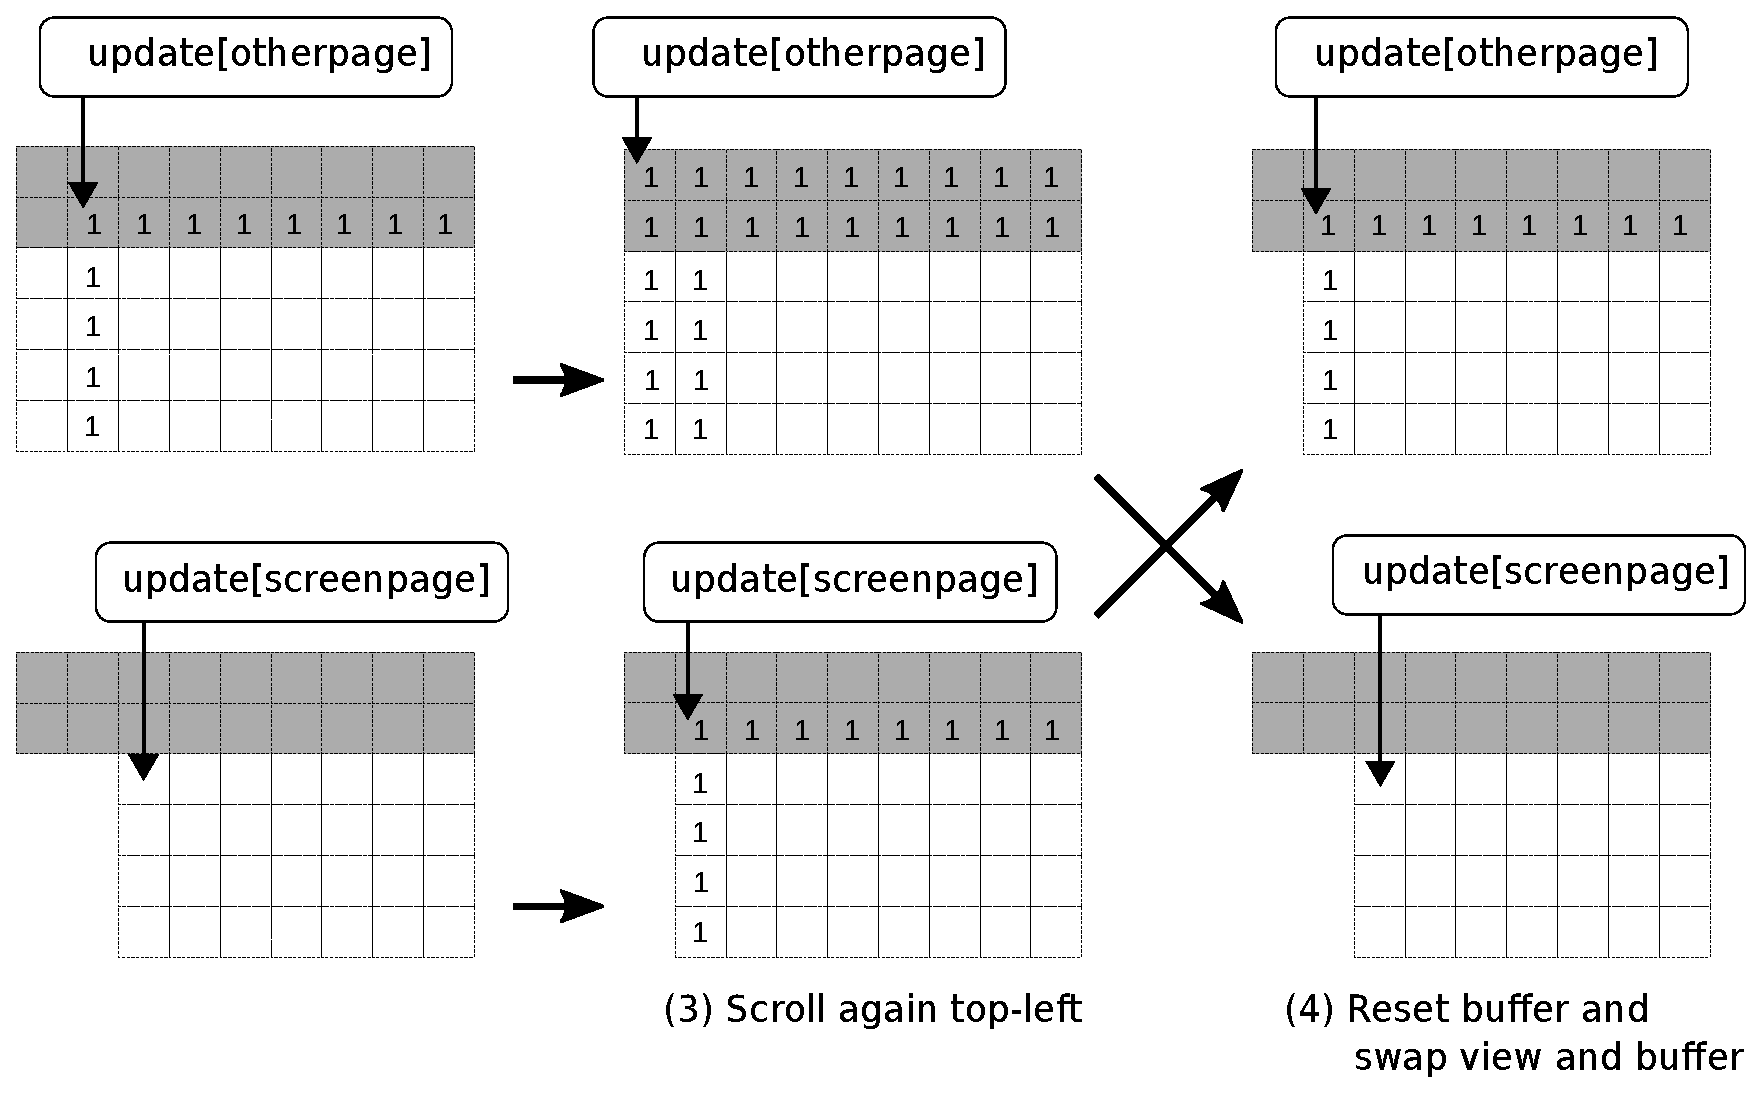
\includegraphics[width=0.85\textwidth]{imgs/drawings/buffer_tile_move_2.eps}
  \caption{scroll to top-left tile again.}
  \label{fig:buffer_tile_move_2}
\end{figure}

\pagebreak

\subsection{Screen refresh}

Flipping between the pages is as simple as setting the CRTC start address registers to page 0 or page 1 starting point. 
However, there is one issue to solve. If you were to run it, every once in a while the expected screen shown below...

 \begin{figure}[H]
\centering
 \scaledimage{0.85}{/game/full_screen.png}
 \end{figure}
...would instead appear distorted:\\
\par
 \begin{figure}[H]
\centering
 \scaledimage{0.85}{/game/crtc_scanstart_problem.png}
 \end{figure}
\par
This glitch shows both misalignment and parts of two pages. This problem has to do with the timing between updating the CRTC starting address and screen refresh. The start address is latched by the EGA's internal circuitry exactly once per frame, typically at the start of the vertical retracement. The CRTC starting address is a 16-bit value but the \cw{out} instruction can only write 8 bits at a time. \\
\par

Now we have the following situation, where the current CRTC start address (Page 0) is pointing to \cw{0x0000} and the buffer (Page 1) to \cw{0x3C00}. We moved one tile to the left and now Page 0 is pointing at 0xFFFE in VRAM and Page 1 is at 0x3BFE. Page 1 is the updated buffer and will be displayed upon next refresh cycle. Poor timing of the vertical retracement and start address update results in the CRTC only picking up the first byte of the address, \cw{0x3B}, and setting the new start address to \cw{0x3B00} instead of \cw{0x3BFE}.\\

\par
\begin{minipage}{\textwidth}
\lstinputlisting[language={[x86masm]Assembler}]{code/pageflip_error.c}
\end{minipage}
\par

The most obvious solution to this issue is to update the start address when we pick up the vertical retracement signal via the Input Status 1 Register (bit 3 of \cw{0x3DA}). Unfortunately, by the time the vertical retrace status is observed by a program, the start address for the next frame has already been latched, having happened the instant the vertical retrace pulse began.\\

\par
The trick is to update the start address sufficient far away from when the vertical retracement starts. So we're looking for a signal that tells us it just finished a horizontal or vertical retrace and started a scan line, far enough away from vertical retrace so we can be sure the new start address will get used at the next vertical sync. This signal is provided by the Display Enable status signal via the Input Status 1 Register, where a value of 1 indicates the display is in a horizontal or vertical retracement\footnote{Documentation is a bit unclear here. The IBM technical documentation for VGA explains retrace takes place when bit 0 of the Input Status Register 1 is set to high ('1'). The IBM technical EGA documentation explains the opposite, saying when bit 0 is set low ('0') a retrace is taking place. For now, we assume source code and VGA documentation is correct, retrace takes place on a '1'.}.
\\

\begin{figure}[H]
  \centering
  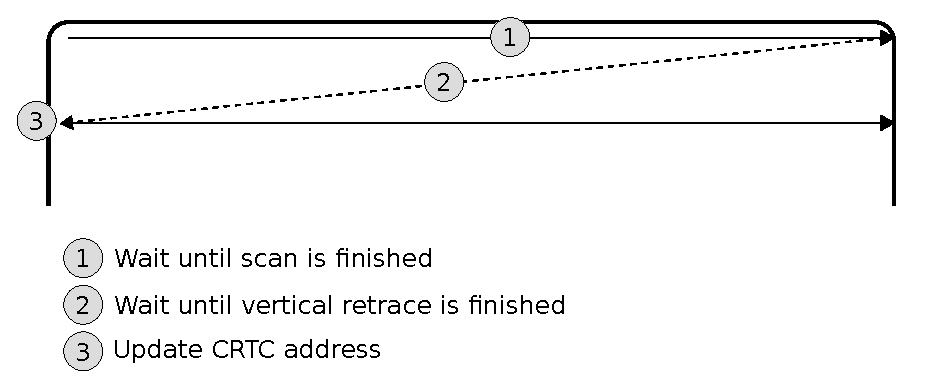
\includegraphics[width=\textwidth]{imgs/drawings/update_start_address.eps}
  \label{fig:update_start_address}
  \caption{Update CRTC start address at beginning of new scan line.}
\end{figure}
\par

When the Display Enable status is observed, the program sets the new start address. Once the CRTC start address is updated, the game waits for vertical retrace to happen, sets the new pel panning state, and then continues drawing.\\
\par
\begin{minipage}{\textwidth}
\lstinputlisting[language={[x86masm]Assembler}]{code/screen_refresh.c}
\end{minipage}
\par




\section{Actors and sprites}

\subsection{A.I.}
To simulate enemies, some objects are allowed to "think" and take actions like walking,
shooting or emitting sounds. These thinking objects are called "actors".
Actors are programmed via a state machine. They can be aggressive (chase you), just running in any direction, or dump (throwing things at you). To model their behavior, all enemies have an associated state:
\begin{itemize}
  \item Chase Keen
  \item Smash Keen
  \item Shoot projectile
  \item Climb and slide from pole
  \item Walking around
  \item Turn into flower
  \item Special Boss (Boobus)
\end{itemize}
\par

Each state has associated think, reaction and contact method pointers. There is also a next
pointer to indicate which state the actor should transition to when the current state is completed.\\
\par
\begin{minipage}{\textwidth}
  \lstinputlisting[language=C]{code/statetype.c}
\end{minipage}
\label{state_type}
\par

All actors have a state chain, as example the tater trooper.\\
\par
\begin{minipage}{\textwidth}
\lstinputlisting[language=C,style=mystyle,basicstyle=\small]{code/s_grdchase.c}
\end{minipage}
\par
All types of enemies (including Boobus) have their own state machine. They often share
the same reactions (e.g. WalkReact and ProjectileReact), but often have their own thinking state.

\subsection{Drawing Sprites}
\label{section:draw_sprites}
Once the state of the actor is updated, it is time to render the actor on the screen. This is done using sprites and contains the following steps:
\begin{enumerate}
\item Update the state and move actors within the active region.
\item Determinate if a actor has changed or moved
\item Update the actor by removing and drawing sprites to it's new position
\end{enumerate}

Unlike many game consoles such as Nintendo, the concept of sprites did not exists on the EGA card, so again the team needs to write their own solution. As explained in Section \ref{section:asset_file_structure} (Page \pageref{table:spritetable}, table \ref{table:spritetable}) each sprite asset contains additional information which is illustrated in Figure \ref{fig:sprite_structure}.\\
\begin{figure}[H]
  \centering
  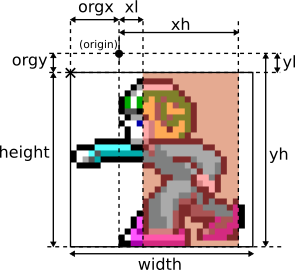
\includegraphics[width=0.6\textwidth]{imgs/drawings/sprite.png}
  \caption{sprite structure}
  \label{fig:sprite_structure}
\end{figure}

All global movement takes place from the origin. The origin is offset by \cw{(orgx, orgy)} from the top-left location of the sprite. The parameters \cw{(xl, xh, yl, yh)} define the hit box of the sprite, which is used to detect collisions.\\

\begin{table}[H]
  \begin{tabularx}{\textwidth}[c]{lXXXXXXXXX}
  \hline
  \textbf{index} & \textbf{width} & \textbf{height} & \textbf{orgx} & \textbf{orgy}
    & \textbf{xl} & \textbf{yl} & \textbf{xh} & \textbf{yh} & \textbf{shift} \\ \hline
  0  &   3  &   24  &   0  &   0  &   0  &   0  &   368  &   368  &   4 \\
  1  &   3  &   32  &   0  &   0  &   64  &   0  &   304  &   496  &   4 \\
  2  &   3  &   30  &   0  &   16  &   64  &   0  &   304  &   496  &   4 \\
  3  &   3  &   30  &   0  &   32  &   64  &   48  &   304  &   496  &   4 \\
  4  &   3  &   32  &   0  &   0  &   64  &   0  &   304  &   496  &   4 \\
  5  &   3  &   30  &   0  &   32  &   64  &   48  &   304  &   496  &   4 \\
 ...  &   ...  &   ...  &   ...  &   ...  &   ...  &   ...  &   ...  &   ...  &   ... \\
 296  &   12  &   103  &   -128  &   0  &   256  &   128  &   752  &   1648  &   4\\
  \end{tabularx}
  \caption{content of spritetable[] in the \cw{KDREAMS.EGA} asset file.}
  \label{table:spritetable}
\end{table}

Once the new state and movement of the actor is calculated from the state machine, the engine needs to first remove the current sprite from the buffer and then redraw the sprite on the new location.\\

\par
Erasing sprites from the buffer page is done by maintaining a list of erase blocks. Each erase block contains the screen (x,y) location, width and height of the sprite to be erased. Instead of copying each variable one-by-one, it makes smartly use of \cw{memcpy} function. \\

\par
\begin{minipage}{\textwidth}
  \lstinputlisting[language=C]{code/sprite_removal.c}
\end{minipage}
\par

The engine is maintaining two list of erase blocks; one for the view page and one for the buffer page. As explained before, each erase block is copying from the (static) master page to the buffer page.\\

\par
As each sprite can float freely over the screen, also here bitshifted sprites are used to position the sprite on a byte-aligned memory layout (as explained in section \ref{section:bitshifting} on page \pageref{section:bitshifting}). The value in the shift column defines the amount of steps the sprite has to be shifted within 8 pixels. A shift value of 4 means the sprite is shifted in 4 steps with a 2 pixel interval.\\ 

\begin{figure}[H]
  \centering
  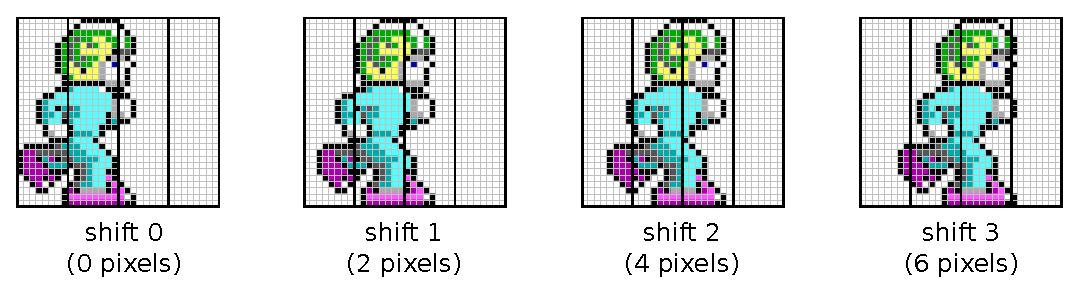
\includegraphics[width=\textwidth]{imgs/drawings/sprite_shift.eps}
  \caption{Sprite shifted in 4 steps.}
  \label{fig:sprite_shift}  
\end{figure}
\par
Displaying the correct shifted sprite is as simple as below.
\\
\par
\begin{minipage}{\textwidth}
  \lstinputlisting[language=C]{code/sprite_shift.c}
\end{minipage}
\label{state_type}
\par


\subsection{Clipping}
\label{section:clipping}
Before drawing a sprite on the screen, the engine determines if the boundaries of a sprite are hitting a wall or floor. This is called clipping and ensures an actor doesn't fall through a floor or walks through a vertical wall. To define whether a tile is a wall or floor, a tile is enriched with tile information, as explained in section \ref{section:foreground_tile_info} on page \pageref{section:foreground_tile_info}. Each foreground tile contains a \cw{NORTHWALL}, \cw{SOUTHWALL}, \cw{EASTWALL} and \cw{WESTWALL}, as explained in section \ref{section:foreground_tile_info}. A number greater than 0 means the tile is a wall or floor when approaching from a given direction. 

\begin{figure}[H]
\centering
\begin{subfigure}{.5\textwidth}
  \centering
  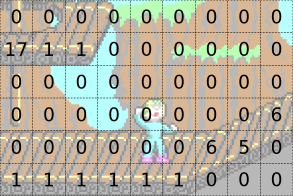
\includegraphics[width=.9\textwidth]{screenshots_300dpi/game/clip_tinf_1.png}
  \caption{Wall type map NORTHWALL}
  \label{fig:clip_tinf_n}
\end{subfigure}%
\begin{subfigure}{.5\textwidth}
  \centering
  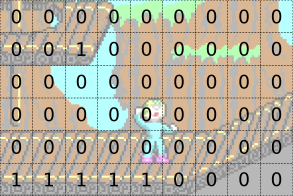
\includegraphics[width=.9\textwidth]{screenshots_300dpi/game/clip_tinf_east.png}
  \caption{Wall type map EASTWALL}
  \label{fig:clip_tinf_e}
\end{subfigure}
\caption{Foreground tile clipping information.}
\label{fig:clip_tinf}
\end{figure}

\par
As example, when a sprite, moving from right to left, is hitting a wall on the left side, it will update the sprite movement to ensure the sprite clips to the east wall of the left tile as illustrated in Figure \ref{fig:clipping_east}. The east/west wall clipping logic is covered by \cw{ClipToEastWalls()} and \cw{ClipToWestWalls()} functions. \\

\begin{figure}[H]
  \centering
  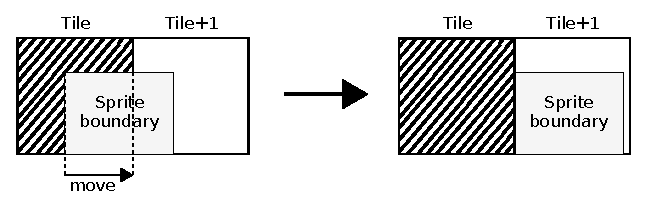
\includegraphics[width=\textwidth]{imgs/drawings/clipping_east.eps}
  \caption{Clipping to east wall when moving from the west.}
  \label{fig:clipping_east}  
\end{figure}

\par
\begin{minipage}{\textwidth}
  \lstinputlisting[language=C]{code/clip_east_wall.c}
\end{minipage}
\label{wallclip_array}
\par
For clipping top and bottom the engine also needs to take clipping to slopes into account. After the sprite is clipped to the top or bottom of the wall tile, an offset can be applied to move a sprite up or down a slope. The offset is defined by a lookup table, where the midpoint of the sprite and the wall type from the foreground tile defines the offset.

\begin{figure}[H]
  \centering
  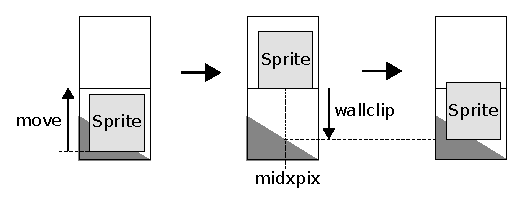
\includegraphics[width=\textwidth]{imgs/drawings/clipping_north.eps}
  \label{fig:clipping_north}
  \caption{Clipping north wall with slope.}
\end{figure}



\begin{minipage}{\textwidth}
  \lstinputlisting[language=C,style=mystyle,basicstyle=\scriptsize]{code/wallclip_array.c}
\end{minipage}
\label{wallclip_array}
\par
\begin{figure}[H]
  \centering
  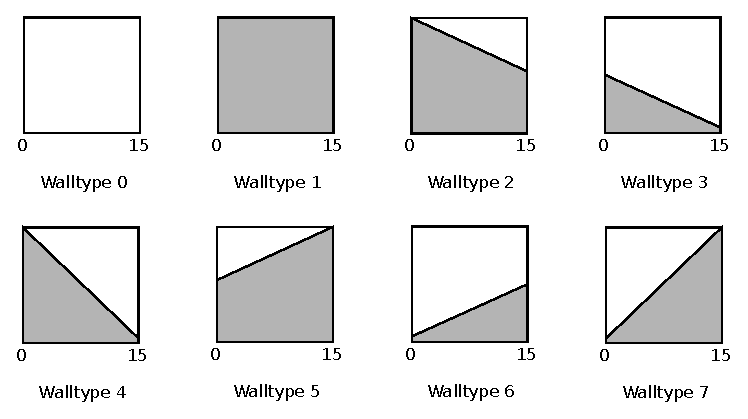
\includegraphics[width=\textwidth]{imgs/drawings/walltype.eps}
  \caption{Eight different walltypes (slopes) defined.}
  \label{fig:walltype}
\end{figure}



\par
\begin{minipage}{\textwidth}
  \lstinputlisting[language=C]{code/clip_north_wall.c}
\end{minipage}
\label{wallclip_array}
\par

\subsection{Priority of tiles and sprites on screen}
The normal screen build is as follows:
\begin{enumerate}
  \item Draw the background tiles.
  \item Draw the masked foreground tiles.
  \item Draw the sprites on top of both the background and foreground tiles.
\end{enumerate}

If multiple sprites are displayed on the same tile, each sprite is given a priority 0-3 to define the order of drawing. A sprite with a higher priority number is always displayed on top of lower priority sprites. As sprites are always displayed on top of tiles, this is causing unnatural situation when Commander Keen is climbing through a  hole as illustrated in Figure \ref{fig:draw_layers}.\\

\begin{figure}[H]
\begin{subfigure}{.25\textwidth}
  \centering
  
\includegraphics[width=.9\textwidth]{screenshots_300dpi/game/tile_composite_1.png}
  \caption{Background tile.}
\end{subfigure}%
\begin{subfigure}{.25\textwidth}
  \centering
  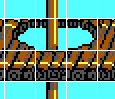
\includegraphics[width=.9\textwidth]{screenshots_300dpi/game/tile_composite_2.png}
  \caption{Foreground tile.}
\end{subfigure}
\begin{subfigure}{.25\textwidth}
  \centering
  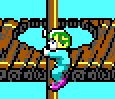
\includegraphics[width=.9\textwidth]{screenshots_300dpi/game/tile_composite_3.png}
  \caption{Sprite on top.}
\end{subfigure}
\caption{Unnatural situation where Commander Keen is in front of a hole.}
\label{fig:draw_layers}
\end{figure}
\par

To draw sprites 'inside' a foreground tile, a small trick is used by introducing a priority foreground tile. As explained in section \ref{section:foreground_tile_info} each foreground tile is enriched with INTILE ('inside tile') information. If the highest bit (\cw{80h}) of INTILE is set, this foreground tile has a higher priority than sprites with a priority 0, 1 or 2. So when drawing the tiles and sprites the following drawing order is applied:
\begin{enumerate}
  \item Draw the background tile.
  \item Draw the masked foreground tile.
  \item Draw sprites with priority 0, 1 and 2 (in that order) and mark the corresponding tile in the tile buffer array with '3' as illustrated in Figure \ref{fig:kc1_3_tile_update_sprite} on page \pageref{fig:kc1_3_tile_update_sprite}.
  \item Scan the tile buffer array for tiles marked with '3'. If the corresponding foreground INTILE high bit (\cw{80h}) is set, redraw the masked foreground tile.
  \item Finally, draw sprites with priority 3. These sprites are always on top of everything.
\end{enumerate}
\par
The priority foreground tiles are updated in the \cw{RFL\_MaskForegroundTiles()} function.\\

\begin{figure}[H]
\centering
\begin{subfigure}[t]{.245\textwidth}
  \centering
  
\includegraphics[width=.9\textwidth]{screenshots_300dpi/game/tile_composite_1.png}
  \caption{Background tile.}
\end{subfigure}%
\begin{subfigure}[t]{.245\textwidth}
  \centering
  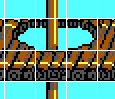
\includegraphics[width=.9\textwidth]{screenshots_300dpi/game/tile_composite_2.png}
  \caption{Foreground tile.}
\end{subfigure}
\begin{subfigure}[t]{.245\textwidth}
  \centering
  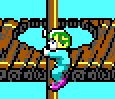
\includegraphics[width=.9\textwidth]{screenshots_300dpi/game/tile_composite_3.png}
  \caption{Sprite on top.}
\end{subfigure}
\begin{subfigure}[t]{.245\textwidth}
  \centering
  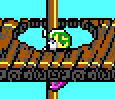
\includegraphics[width=.9\textwidth]{screenshots_300dpi/game/tile_composite_4.png}
  \caption{Redraw masked foreground tile.}
\end{subfigure}
\caption{Draw sprite inside a tile, by redrawing foreground tile.}
\label{fig:clip_tinf}
\end{figure}

\par
\begin{minipage}{\textwidth}
  \lstinputlisting[language={[x86masm]Assembler}]{code/mask_foreground_tile.asm}
\end{minipage}
\label{mask_foreground_tile}
\par

\subsection{Manage refresh timing}
After each screen refresh a certain amount of time, which we call ticks, has passed. The amount of ticks depends on several factors like amount of tiles refreshed and waiting time for a screen vertical retrace. Since all game actions and reactions rely on the amount of ticks between two refreshes, it is important to keep the tick interval consistent.\\

\par
Without controlling the tick interval, the state and speed of actors could become unreliable, they could run faster and even can "warp" to an unexpected location. To control refresh intervals, a minimum and maximum number of tics is defined in the refresh loop.\\

\par
\begin{minipage}{\textwidth}
  \lstinputlisting[language=C]{code/time_ticks.c}
\end{minipage}
\label{time_ticks}
\par

\pagebreak

The game and all actors are defined in a global coordinate system, which is scaled to 16 times a pixel. The higher resolution enables more precision of movements and better simulation of movement acceleration. Conversion between global and pixel coordinatess can be easily performed by bit shift operations.\\
\section{use later}
\begin{minipage}{\textwidth}
  \lstinputlisting[language=C]{code/EGA_REFRESH.ASM}
  \end{minipage}
  \label{ega_refresh}
  \par

\section{ATR}


In the file \cw{id\_vw.h} the virtual screen in VRAM is defined by SCREENSPACE, which is set to 512x240 pixels (64x240 = 15,360 bytes). This is more than sufficient since the visible screen in mode \cw{0x0D} is 320x200 pixels.\\

Since one screen only uses 15,360 bytes of VRAM (which is 3,840 bytes per plane), there is more than enough space to store more than two full screens of video data. 

\par
Before explaining the scrolling algorithm, let's first explain how the tile layout is organized. The EGA screen in mode \cw{0xD} has a resolution of 320x200 pixels. Translated in 16x16 pixel tiles, the screen view has a size of 20x13 tiles (actually 12.5 tiles high, but we round up to 13 tiles). By making the port view one tile higher and wider than the screen, the engine can scroll the screen up to 16 pixels to the right or bottom side of the screen without any tile refresh, by means of adjusting the CRTC Start Address and Pel Pan registers. Finally, the buffer must have enough space to float the view port up to two tiles in all directions (This is required for later versions of Commander Keen, which will be explained in Section \ref{section:scroll_refresh_dreams}). In total two tile arrays are maintained; one for the view screen and one for the buffer screen.\\
\par
 
\begin{figure}[H]
\centering
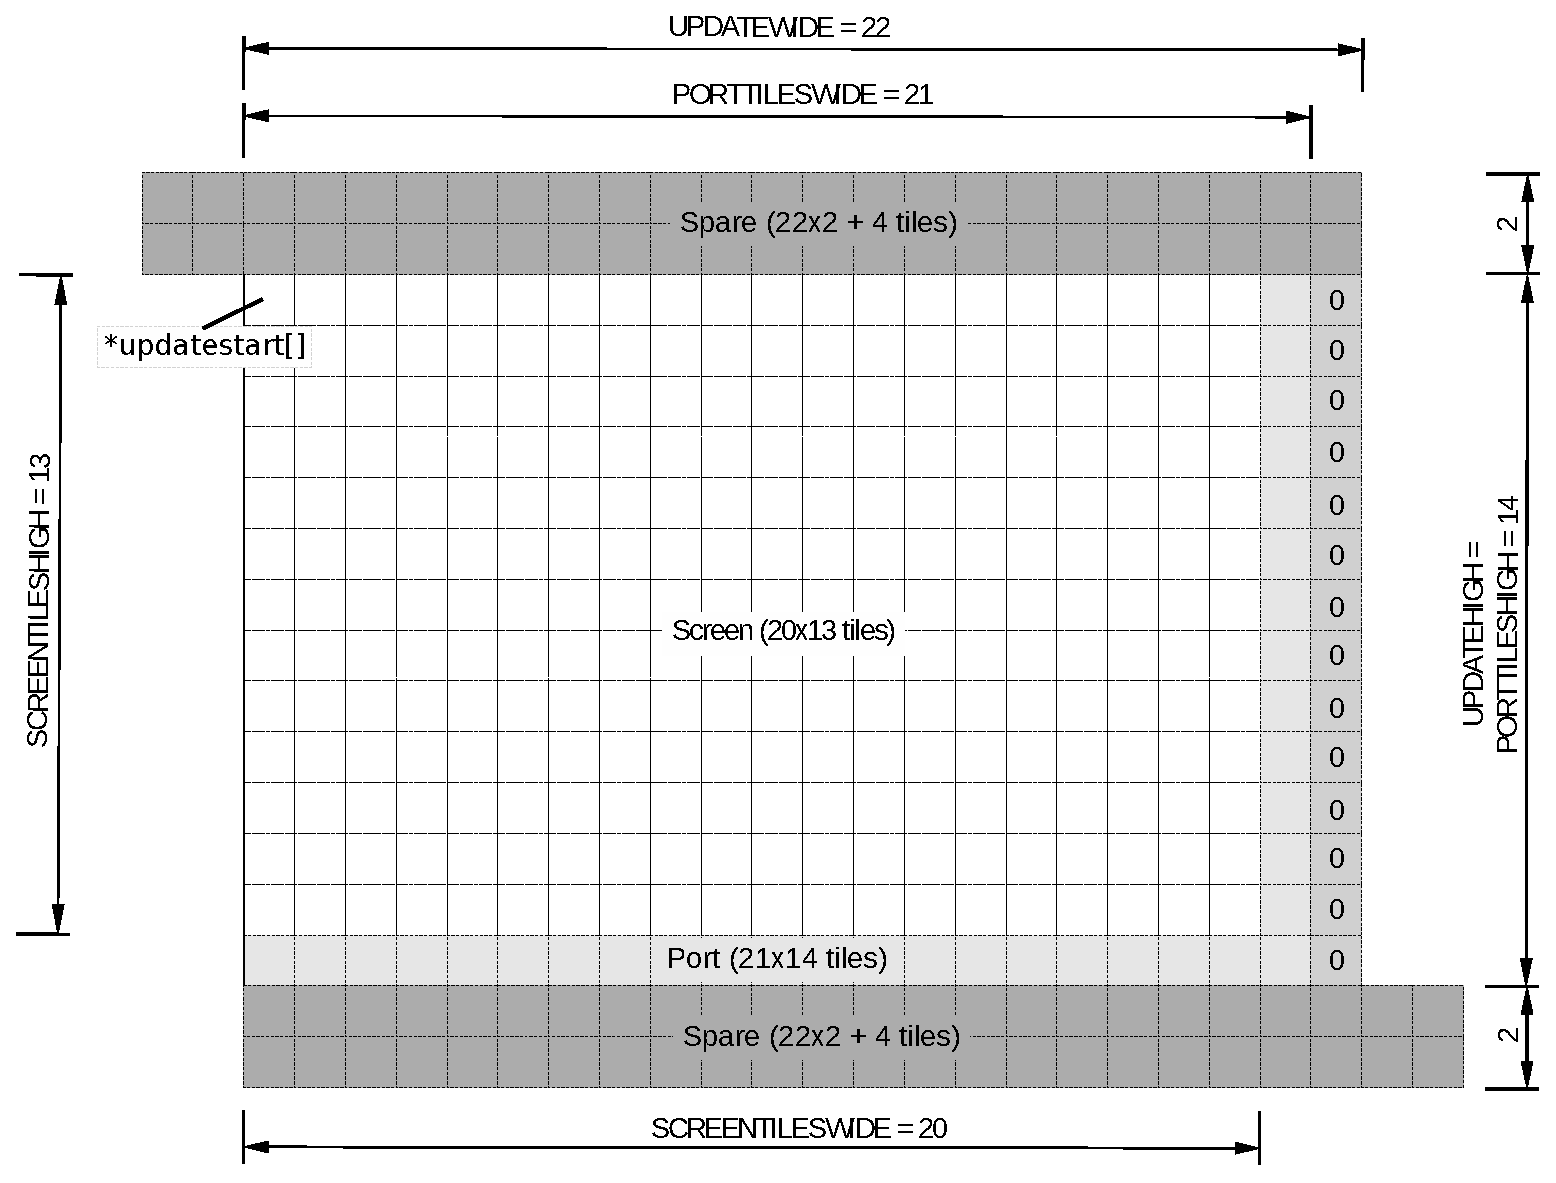
\includegraphics[width=\textwidth]{imgs/drawings/buffer_tile_layout.eps}
\caption{Tile view and tile buffer layout.}
\label{fig:screen_setup}
\end{figure}





\subsection{Adaptive tile refreshment in Commander Keen 1-3}
In the this section we explain how the first 3 versions of the game are working\footnote{We can only explain how the algorithm is working without code examples, since the only released code is Keen Dreams which is using the improved algorithm.}. Six stages are involved in drawing a 2D scene:
\begin{enumerate}
\item Check if the player has moved one tile in any direction.
\item Validate which tiles have changed (both from scrolling and animated tiles), copy these respective tiles to the master page and mark the tiles in both tile arrays (view and buffer tile arrays).
\item Refresh the buffer page by scanning all tiles. If a tile needs to be updated, copy the tile from the master page to the buffer page.
\item Iterate through the sprite removal list and copy corresponding image block from the master page to buffer page. 
\item Iterate through the sprite list and copy corresponding sprite image block from RAM to buffer page.
\item Switch the view and buffer page by adjusting the CRTC Start Address and Pel Panning registers.
\end{enumerate}



In the next six screenshots, we take you step-by-step through each of the stages. The player has moved and forces the screen to scroll one tile to the right. \\

\end{document}